\documentclass[
11pt, % The default document font size, options: 10pt, 11pt, 12pt
%codirector, % Uncomment to add a codirector to the title page
]{charter} 




% El títulos de la memoria, se usa en la carátula y se puede usar el cualquier lugar del documento con el comando \ttitle
\titulo{Sistema de información visual para pasajeros de Trenes Argentinos} 

% Nombre del posgrado, se usa en la carátula y se puede usar el cualquier lugar del documento con el comando \degreename
\posgrado{Carrera de Especialización en Sistemas Embebidos} 
%\posgrado{Carrera de Especialización en Internet de las Cosas} 
%\posgrado{Carrera de Especialización en Intelegencia Artificial}
%\posgrado{Maestría en Sistemas Embebidos} 
%\posgrado{Maestría en Internet de las cosas}

% Tu nombre, se puede usar el cualquier lugar del documento con el comando \authorname
\autor{Ing. Carlos German Carreño Romano} 

% El nombre del director y co-director, se puede usar el cualquier lugar del documento con el comando \supname y \cosupname y \pertesupname y \pertecosupname
\director{Dr. Ing. Pablo Gomez}
\pertenenciaDirector{FIUBA} 
% FIXME:NO IMPLEMENTADO EL CODIRECTOR ni su pertenencia
%\codirector{} % para que aparezca en la portada se debe descomentar la opción codirector en el documentclass
%\pertenenciaCoDirector{}

% Nombre del cliente, quien va a aprobar los resultados del proyecto, se puede usar con el comando \clientename y \empclientename
\cliente{Trenes Argentinos Operaciones, Operadora Ferroviaria S.E.  (SOFSE)}
\empresaCliente{Empresa del cliente}

% Nombre y pertenencia de los jurados, se pueden usar el cualquier lugar del documento con el comando \jurunoname, \jurdosname y \jurtresname y \perteunoname, \pertedosname y \pertetresname.
\juradoUno{Nombre y Apellido (1)}
\pertenenciaJurUno{pertenencia (1)} 
\juradoDos{Nombre y Apellido (2)}
\pertenenciaJurDos{pertenencia (2)}
\juradoTres{Nombre y Apellido (3)}
\pertenenciaJurTres{pertenencia (3)}
 
\fechaINICIO{30 de Marzo de 2020}		%Fecha de inicio de la cursada de GdP \fechaInicioName
\fechaFINALPlan{15 de Junio de 2021} 	%Fecha de final de cursada de GdP
\fechaFINALTrabajo{12 de Diciembre de 2021}	%Fecha de defensa pública del trabajo final


\begin{document}

\maketitle
\thispagestyle{empty}
\pagebreak


\thispagestyle{empty}
{\setlength{\parskip}{0pt}
\tableofcontents{}
}
\pagebreak


\section*{Registros de cambios}
\label{sec:registro}


\begin{table}[ht]
\label{tab:registro}
\centering
\begin{tabularx}{\linewidth}{@{}|c|X|c|@{}}
\hline
\rowcolor[HTML]{C0C0C0} 
Revisión & \multicolumn{1}{c|}{\cellcolor[HTML]{C0C0C0}Detalles de los cambios realizados} & Fecha      \\ \hline
0      & Creación del documento                                 &\fechaInicioName \\ \hline
%1      & Se completa hasta el punto 4 inclusive                 & dd/mm/aaaa \\ \hline
%2      & Se completa hasta el punto 7 inclusive
%		  Se puede agregar algo más \newline
%		  En distintas líneas \newline
%		  Así                                                    & dd/mm/aaaa \\ \hline
%3      & Se completa hasta el punto 11 inclusive                & dd/mm/aaaa \\ \hline
%4      & Se completa el plan	                                 & dd/mm/aaaa \\ \hline
\end{tabularx}
\end{table}

\pagebreak



\section*{Acta de constitución del proyecto}
\label{sec:acta}

\begin{flushright}
Buenos Aires, \fechaInicioName
\end{flushright}

\vspace{2cm}

Por medio de la presente se acuerda con el Ing. \authorname\hspace{1px} que su Trabajo Final de la \degreename\hspace{1px} se titulará ``\ttitle'', consistirá esencialmente en el diseño y fabricación de un prototipo para el control de información visual para pasajeros, y tendrá un presupuesto preliminar estimado de 600 hs de trabajo y \textcolor{red}{\$XXX} de materiales, con fecha de inicio \fechaInicioName\hspace{1px} y fecha de presentación pública \fechaFinalName.

Se adjunta a esta acta la planificación inicial.

\vfill

% Esta parte se construye sola con la información que hayan cargado en el preámbulo del documento y no debe modificarla
\begin{table}[ht]
\centering
\begin{tabular}{ccc}
\begin{tabular}[c]{@{}c@{}}Ariel Lutenberg \\ Director posgrado FIUBA\end{tabular} & \hspace{2cm} & \begin{tabular}[c]{@{}c@{}}\clientename \\ \empclientename \end{tabular} \vspace{2.5cm} \\ 
\multicolumn{3}{c}{\begin{tabular}[c]{@{}c@{}} \supname \\ Director del Trabajo Final\end{tabular}} \vspace{2.5cm} \\
%\begin{tabular}[c]{@{}c@{}}\jurunoname \\ Jurado del Trabajo Final\end{tabular}     &  & \begin{tabular}[c]{@{}c@{}}\jurdosname\\ Jurado del Trabajo Final\end{tabular}  \vspace{2.5cm}  \\
%\multicolumn{3}{c}{\begin{tabular}[c]{@{}c@{}} \jurtresname\\ Jurado del Trabajo Final\end{tabular}} \vspace{.5cm}                                                                     
\end{tabular}
\end{table}


\pagebreak


\section{Introducción}
\label{sec:intro}
\subsection{Introducción específica}
El objetivo de este trabajo es desarrollar y fabricar controladores para el sistema de información visual de pasajeros (PIDS) de Trenes Argentinos (SOFSE). Este sistema se presenta al pasajero a través de carteles LED de salón que dan mensajes como la próxima estación, junto con los carteles de frente y contrafrente del tren que indican el ramal destino, como se muestra en la figura 1. 

\begin{figure}[htpb]
\centering 
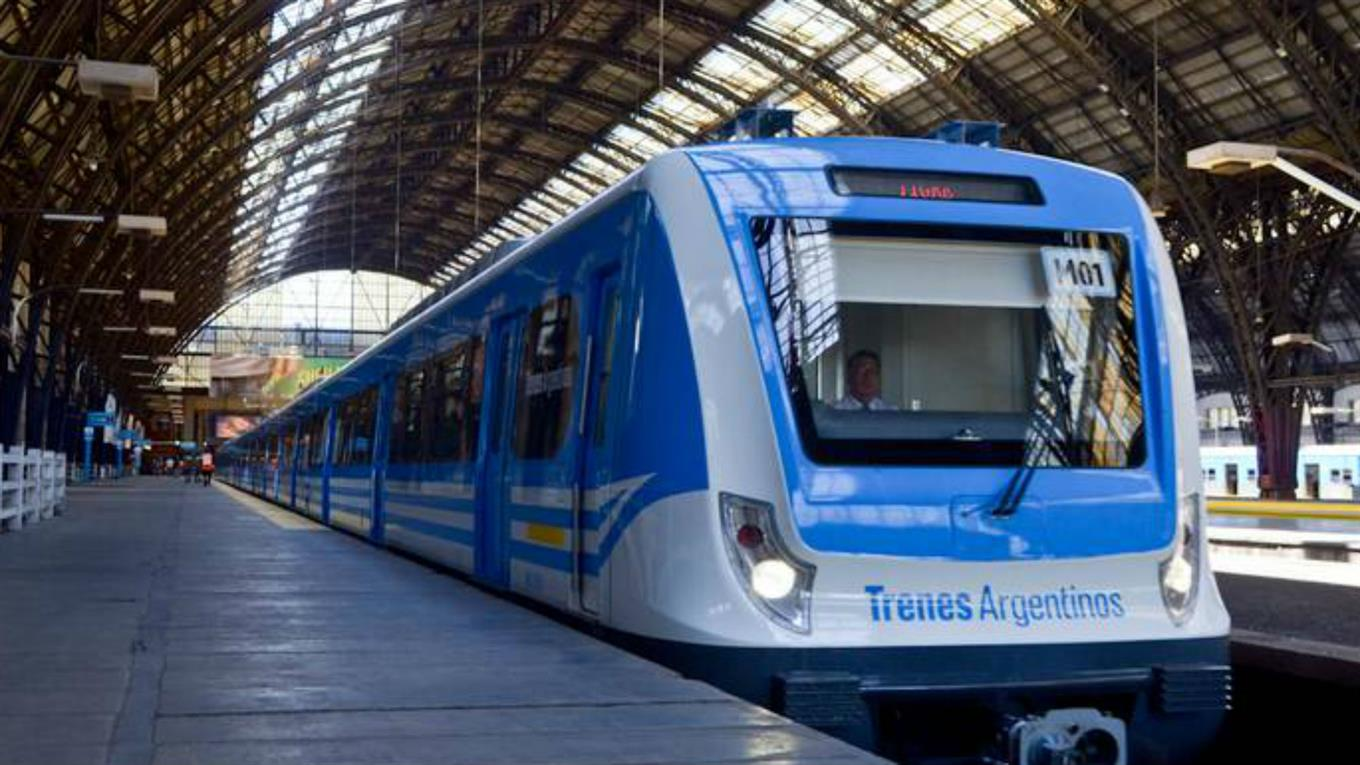
\includegraphics[width=.75\textwidth]{./Pics/tren.jpg}
\caption{Coche cabecera con la marquesina frontal que indica el destino Tigre.}
\label{fig:cartelFrente}
\end{figure}

El potencial de este trabajo es fabricar placas de control que permitan al personal de trenes realizar reparaciones y sustituir importaciones, obteniendo como resultado un mejor servicio de cara al usuario y mayor independencia tecnológica.

El desafío principal del proyecto es la compatibilidad con la red de comunicación del tren (TCN) existente. Las placas de control deben poder generar información en carteles LED y a la vez interconectarse a la red TCN. La posibilidad de fabricar el equipamiento en la industria local es también un desafío central de este proyecto.

\pagebreak

\section{Planificación}

\pagebreak

\section{Diseño}

\subsection{Display LED}
La placa de control del display LED matricial se representa con el diagrama de bloques de la figura \ref{fig:blockDiagram LED display}. La entrada es un conector de dieciséis pines (2x8) que entrega señal de datos a dos transceivers 74HC245D. El circuito de los transceivers s

\begin{figure}[htpb]
\centering 
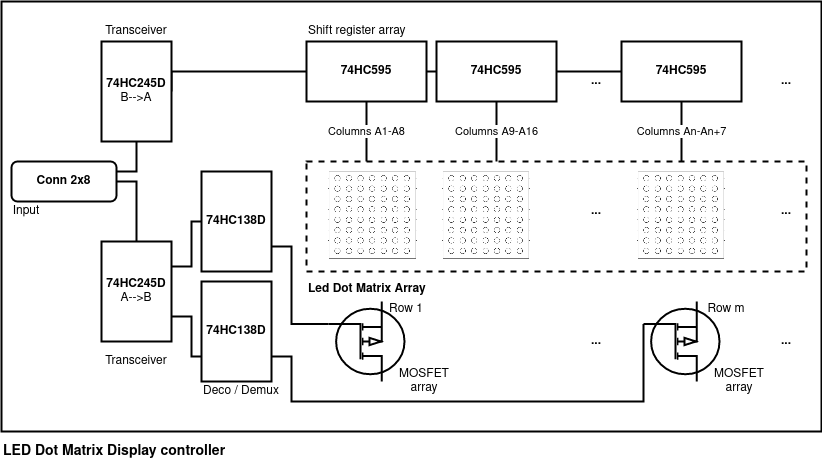
\includegraphics[width=1\textwidth]{./Pics/blockDiagram.png}
\caption{Diagrama de bloques del controlador del display LED.}
\label{fig:blockDiagram LED display}
\end{figure}

\subsection{Controlador}

\section{Fabricación}
\section{Pruebas}
\section{Integración}

\end{document}


El sistema PIDS tiene la capacidad de presentar diversos mensajes de información al pasajero, como por ejemplo el nombre de la próxima estación, la temperatura actual, el tiempo estimado de arribo a destino, entre otros. Los mensajes se visualizan en carteles LED de 120 cm x 30 cm aproximadamente, usando matrices de punto LED de un solo color. La placa de control es compatible con manejadores de carteles LED comerciales, y también es compatible con la red eléctrica de 110 VDC del tren. El PIDS además cuenta con varios módulos adicionales, como son el sistema de sonido y el sistema de video entre otros. Cada módulo se compone de piezas de hardware específicas, distribuidas e interconectadas a lo largo del tren. En la figura \ref{fig:diagBloques} se presenta un diagrama de bloques del sistema PIDS. Se resalta en color los módulos de control incluidos en el alcance de este proyecto.

%\vspace{25px}

\begin{figure}[htpb]
\centering 
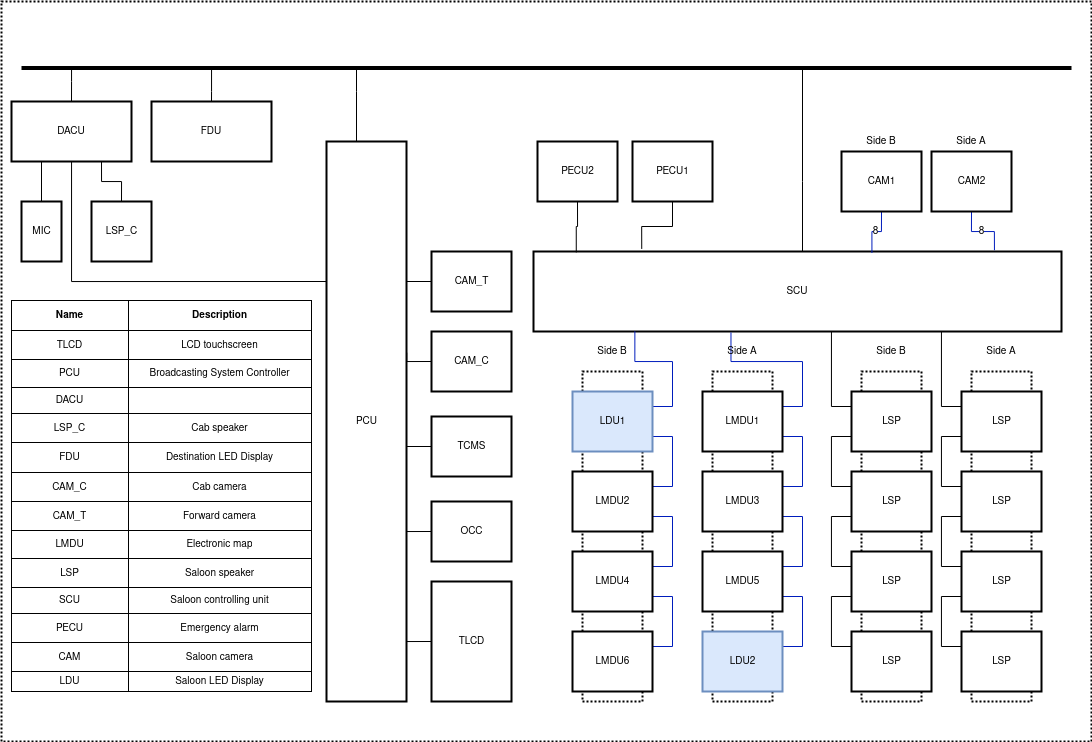
\includegraphics[width=.99\textwidth]{./Pics/RedPIDS.png}
\caption{}
\label{fig:diagBloques}
\end{figure}

\vspace{25px}

Este sistema también ofrece al personal técnico de SOFSE la capacidad de reemplazar placas existentes con alguna falla, configurar el nombre de distintos ramales usando el mismo hardware, y sirve de maqueta para capacitaciones.

Se propone en este trabajo diseñar y fabricar el controlador siguiendo las normas 50155 y 50126. La norma EN 50155 es la norma internacional que rige todos los equipos electrónicos de control, regulación, protección y suministro que se instalan en los vehículos ferroviarios. La norma EN 50126 define el ciclo de vida como: “estructura para la planificación, la gestión, el control y la supervisión de todos los aspectos de un sistema, incluido la fiabilidad, la disponibilidad, la mantenibilidad y la seguridad (RAMS), para entregar el producto adecuado al precio correcto dentro del plazo acordado.”


Este trabajo es continuación del trabajo final de la Carrera de Especialización en Sistemas Embebidos titulado Sistema de información visual para pasajeros, que se enmarca en un Proyecto de Desarrollo Estratégico (PDE), 'PDE\_15\_2020' de UBACyT titulado como “Sistema de monitoreo y gestión de la red TCN en formaciones ferroviarias”

\label{sec:backlog}

\subsection{UC-1} 
Como usuario quiero visualizar el nombre de la estación arribada.

\textbf{Descripción:} El sistema genera un mensaje que contiene información para el pasajero y se lo presenta en una marquesina LED.

\textbf{Disparadores:} El evento se inicia cuando el tren arriba a una 
estación.


